This chapter contains the detailed design of the receiver satellites. Each section contains the final design of a different subsystem. 
\\\\
The most important subsystem is the optical receivind payload found in section \ref{sec:DDreceiver}. The navigation and satellite position is discussed in section \ref{NaviReceiver}. Thirdly the inter-satellite and space-ground communication is explained in detail in section \ref{sec:comm_receiver}. Section \ref{recDDadcs} contains the detailed design of the \ac{ADCS}. The power generation and the corresponding power system is documented in section \ref{receiver_EPS}. 
\\\\
Figure \ref{fig:receiverSat} shows an impression of what the receiver satellites will look like.

\begin{figure}
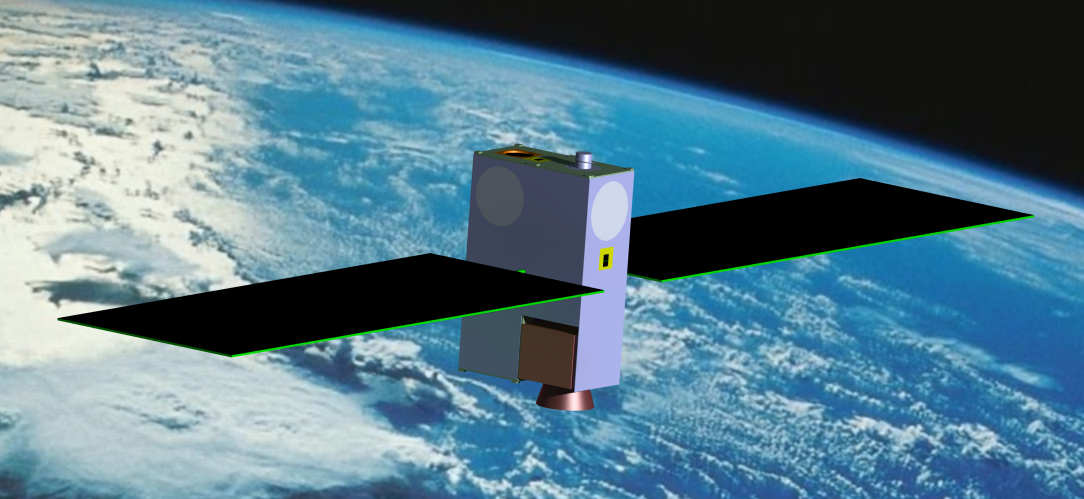
\includegraphics{chapters/img/receiver.tif}
\caption{Impression of the receiver satellites}
\label{fig:receiverSat}
\end{figure}